\chapter{Outlook} \label{chap:Outlook}
This chapter outlines important aspects that should be considered when further realizing an Ethernet-based implementation for a Distributed Test Support System.

\section{Implementation in the DML}
Since the investigations have shown that a UDP-based solution is feasible, the next step is to implement it in the \acf{dml} (see \ref{chap:DML}). This will be done by the author after the thesis.

This involves replacing the \ac{fifo} buffers in the \ac{dml} for the remote nodes with UDP sockets. The Data Manager will then poll these sockets instead of the \ac{fifo} buffers. In addition, data transmission to remote nodes of the Distributed Test Support System must also be implemented using sockets instead of \ac{dma}.

After implementation, extensive testing with the UDP-based \ac{dml} solution should be performed.

\section{Detection of Network Overload}
According to the key results (see Chapter \ref{chap:KeyResults}), high network loads can have a negative impact on the reliability and performance of computer systems. To inform the user of the Test Support System that the system is operating at a load limit and degradation might be experienced, a network overlaod detection mechanism should be implemented.

This mechanism could be implemented in the Data Manager of the \ac{dml}. A possible solution is to monitor the average throughput of all UDP communications of the system and to issue a warning message to the user at a certain threshold, which depends on the type of system.

\section{Fragmentation Algorithm based on UDP} \label{chap:fragProposalOutlook}
In the Distributed Test Support System, messages exchanged through the DML may exceed the maximum datagram size of the UDP protocol of 65,515 bytes. To transmit these messages using a UDP socket, a fragmentation algorithm must be implemented by the application.

Based on the results of the investigation that unfragmented UDP datagrams are not reordered in a local network without a switch, the information required for fragmentation and defragmentation can be significantly reduced compared to the IP protocol (see \ref{chap:frag}). A proposal for a fragmentation mechanism is outlined below.

\begin{figure}[h!]
    \centering
    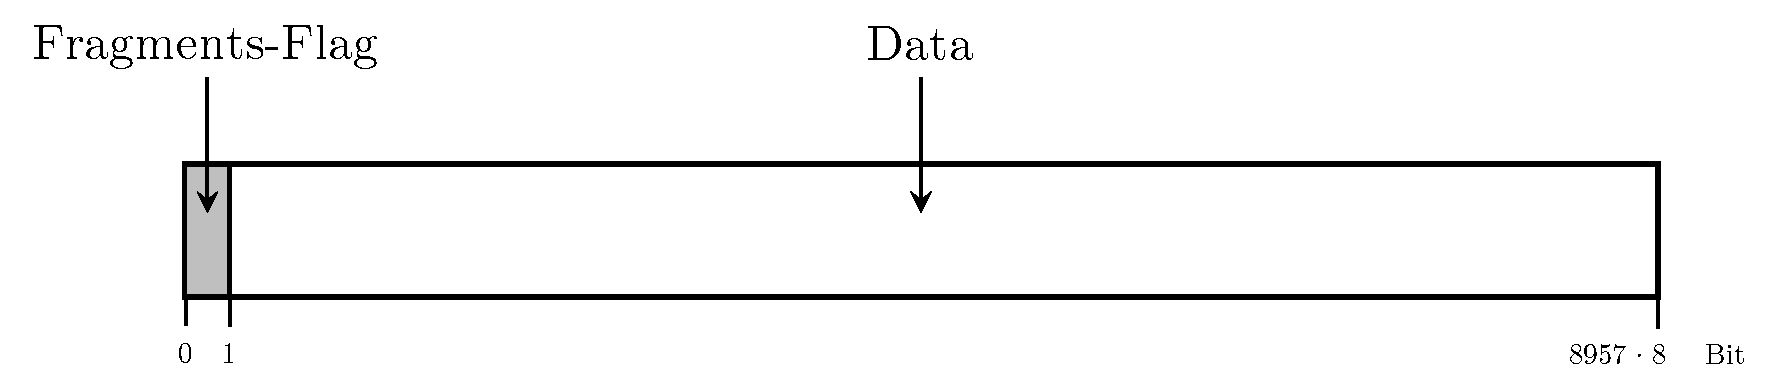
\includegraphics[width=1\linewidth]{figures/outlook/frag_header.pdf}
    \caption{Proposed Header for the Implementation of a Fragmentation Mechanism}
    \label{fig:FragProposal}
\end{figure}

Figure \ref{fig:FragProposal} shows the proposed header format for the implementation of a fragmentation mechanism. The header is 4 bytes in size and is followed by the payload. The maximum payload size for a message passed to the UDP socket is determined by the \ac{mtu}, as the IP protocol should not perform any fragmentation. For an \ac{mtu} of 9000 Bytes, the maximum payload size is 8968 bytes. Equation \ref{eq:PayloadSize} illustrates the calculation.

\begin{alignat}{2}
&\text{Maximum Payload} &&= 9000\ \text{Bytes \textit{(\ac{mtu})}} \label{eq:PayloadSize}\\
&&&\phantom{=}\ - 20\ \text{Bytes \textit{(IP Header)}} \notag \\
&&&\phantom{=}\ - \phantom{0}8\ \text{Bytes \textit{(UDP Header)}} \notag \\
&&&\phantom{=}\ - \phantom{0}4\ \text{Bytes \textit{(Fragmentation Header)}} \notag \\
&&&= 8968\ \text{Bytes} \notag
\end{alignat}

The proposed fragmentation header (see Figure \ref{fig:FragProposal}) includes the following information:

\begin{itemize}
  \item \textbf{Message Identifier} \textit{(2 Bytes)}: The Message Identifier is a sequential number assigned to each message by the sender. All message fragments share the same identifier.
  \item \textbf{Fragment Index} \textit{(1 Byte)}: The Fragment Index is used to number the individual fragments of a message.
  \item \textbf{Fragment Flag} \textit{(1 Bit)}: The Fragment Flag indicates whether the message is fragmented and more fragments will follow.
\end{itemize}

The maximum size that can be handled by this proposed fragmentation algorithm is limited by the \textit{Fragment Index}. Since this field has a size of 1 byte, it can represent 256 different values. Therefore, a message can be divided into a maximum of 256 fragments. Each fragment has a maximum payload of 8968 bytes (see Equation \ref{eq:PayloadSize}), resulting in a maximum message size of $256 \times 8968$ Bytes $= 2,295,808$ Bytes.

The \textit{Fragments Flag} is set by the sender to allow the defragmentation of a message. The flag should not be set for unfragmented messages. For fragmented messages, the flag should be set for all fragments except the last one. This allows the recipient to recognize the individual message fragments and reassemble them into a complete message. The absence of the flag on the last fragment indicates that all parts of the message have been received and defragmentation can be initiated.

The proposed mechanism also allows the detection of errors. The loss of a message, whether fragmented or unfragmented, can be detected using the \textit{Message Identifier}. The \textit{Fragment Index} can be used to detect the loss of fragments of a message.

Additionally, the proposed header format includes 7 unused bits that are available for possible future extensions.


\section{Reduction of Latency with DPDK}
\ac{dpdk} is a collection of software libraries and drivers that enable the processing of network traffic directly in user space. This reduces latency and increases throughput by eliminating context switches between user space and kernel space, as well as the overhead of the standard Linux network stack \cite{outl02}.

Emmerich et al. found in \cite{outl01} that using \ac{dpdk} reduces latency compared to the standard Linux network stack. A substantial reduction was observed, especially in worst-case scenarios.